\graphicspath{{./images},{./monsters/Hemovoric_Venomite/images}}

\MonsterSheetGeometry

% --------------------------------------------------------------------------------------------------- %
% ################################################################################################### %
% #-#-#-#-#-#-#-#-#-#-#-#-#-#-# Monster-Sheet with two Smaller Pictures #-#-#-#-#-#-#-#-#-#-#-#-#-#-# %
% ################################################################################################### %
% --------------------------------------------------------------------------------------------------- %

\chapter*{Hemovoric Venomite}
\stepcounter{chapter}
\addcontentsline{toc}{chapter}{\protect\numberline{\thechapter}Hemovoric Venomite}

\entryfont \noindent \DndDropCapLine{C}rawling silently through the dark recesses of its domain, the Hemovoric Venomite is a small and sinister creature that belongs to the monstrosity category. With a predominantly red body adorned with bone-like features, this insidious predator strikes fear into the hearts of those unfortunate enough to encounter it. Its crawling form resembles a mite, equipped with multiple agile legs that scuttle with eerie precision, allowing it to navigate the most confined spaces effortlessly, whereas its flying form represents more that of a mosquito.

The very sight of the Hemovoric Venomite sends a shiver down the spine. Its grotesque visage features not one, but two mouths - a larger one positioned above the other. The larger mouth dominates its face, sporting skull-like or bone-like characteristics, while the smaller mouth lies beneath, ready to latch onto prey with razor-sharp precision. Bony mandible-like structures protrude from its head, adding to its macabre appearance. Its legs, too, are adorned with these bone-like features, giving the impression of an otherworldly creature emerging from the darkest depths.

But it is the Hemovoric Venomite's insatiable thirst for blood that truly sets it apart. With a predatory instinct honed to perfection, this crawling creature feeds on the life force of its victims. Its teeth-filled mouths or needle-like beak are specially designed to pierce flesh and draw forth the crimson essence that sustains it. While primarily a ground-dweller, the Hemovoric Venomite is a master of stealth, using its diminutive size and uncanny agility to stalk its prey undetected. It waits patiently, hidden in the shadows, before striking with ruthless efficiency.

Encounters with the Hemovoric Venomite are terrifying ordeals. The eerie silence is broken only by the soft scuttling of its legs as it closes in on its unsuspecting quarry. Its ability to blend seamlessly into the darkness and its relentless pursuit make it a formidable foe. Many have fallen victim to its vampiric nature, their life force drained away by the relentless feeding of this nightmarish creature.

Beware the Hemovoric Venomite, for it is a symbol of unyielding hunger and relentless predation, lurking in the deepest shadows, waiting for its next opportunity to sate its insatiable thirst for blood.

\MonsterGraphicAndShortInfo{shortinfo}% shortinfo or none for no Short-Info Box
{%
	{4.25cm}% Shift Horizontal Short Info Box
	{0.5cm}% Shift Vertical Short Info Box
	{-25}% Rotation Angle Short Info Box
	{5cm}% Width of Short-Info Box
	{3}% Number of Lines in Textbox (might be adjusted after 1 compile) 
	{%
		Do not underestimate a single mite, for within the shadows, many stalk silently, their bloodthirst unyielding. %
	}%
}%
{0.4cm}% Shift Horizontal Monster Grpahic
{0.9cm}% Shift Vertical Monster Grpahic
{, anchor=south west}% Further Picture Placement Options
{(current page.south west)}% Anchor-Point on Page
{height=210pt}% Dimension of Graphic
{Hemovoric_Venomite.png}%
\addImageDBEntry{Page 1}{Art}{https://www.artofmtg.com/art/skrelv-defector-mite/}{Skrelv, Defector Mite MtG Art from Phyrexia: All Will Be One}{Brian Valeza}%

\vfill\eject % cammand to break to next column

\MonsterVariant%
	{-2em}% offset to top of page for image
	{Winged_Hemovoric_Venomite.png}% image above Info-Box
	{-1.75cm} % distance offset from image to Variant Box
	{Winged Hemovoric Venomite}% Name of the variant
	{%
		This black-red mosquito-like creature with tattered wings traded in its strong bony-like features and two mouths for a needle-like beak and red tattered wings with which it can fly.
		\DndMonsterAction{Speed}
		30 ft., fly 40 ft.
		\DndMonsterAction{Flyby Attack}
		The Winged Hemovoric Venomite doesn't provoke opportunity attacks when it flies out of an enemy's reach.
		\DndMonsterAction{Sting}
		Melee Weapon Attack: +5 to hit, reach 5 ft., one target. Hit: \DndDice{1d4 + 3} piercing damage. On a successful sting attack, the target must make a DC 12 Constitution saving throw. On a failed save, the target takes \DndDice{2d6} poison damage and is infected with a disease (The disease's effects are at the DM's discretion).
	}% Monster Variant Info
\addImageDBEntry{Page 1}{Art}{https://www.artofmtg.com/art/pestilent-syphoner/}{Pestilent Syphoner MtG Art from Phyrexia: All Will Be One}{Brian Valeza}%

% Monster stat block
\begin{DndMonster}[width=0.5\textwidth]{Hemovoric Venomite}
    \DndMonsterType{Small Monstrosity, neutral evil}

    % If you want to use commas in the key values, enclose the values in braces.
    \DndMonsterBasics[
        armor-class = {14 (natural armor)},
        hit-points  = {\DndDice{6d6 + 6}},
        speed       = {30 ft., climb 30 ft.},
    ]

    \DndMonsterAbilityScores[
        str = 10,
        dex = 16,
        con = 12,
        int = 6,
        wis = 10,
        cha = 6,
    ]

    \DndMonsterDetails[
        %saving-throws = {Str +0, Dex +0, Con +0, Int +0, Wis +0, Cha +0},
        skills = {Perception +2, Stealth +7},
        %damage-vulnerabilities = {cold},
        %damage-resistances = {bludgeoning, piercing, and slashing from nonmagical attacks},
        %damage-immunities = {cold},
        senses = {Darkvision 60ft., Passive Perception 12},
        %condition-immunities = {frightened, poisoned},
        languages = {Common, understands but doesn't speak any languages},
        challenge = 1,
    ]
    
    \DndMonsterAction{Blood Drain}
    Whenever the Hemovoric Venomite makes a successful Bite or Sting attack it regains hitpoints equal to half the damage dealt by the attack.
    
    \DndMonsterAction{Bone Armor}
    The bony features on its head and legs provide it with natural armor, granting it a +2 bonus to AC.
    
    \DndMonsterAction{Shadow Cloak}
    When in dim light or darker areas the Hemovoric Venomite's presence becomes obscured from magical and non-magical senses alike. It gains advantage on saving throws against spells and effects that would reveal its location or presence through divination or scrying.
    
    \DndMonsterAction{Skewering Mandibles}
    On a successful bite attack, the Hemovoric Venomite can attempt to skewer and impale the target. The target must make a DC 12 Dexterity saving throw or take an additional \DndDice{1d10} piercing damage.
	
	\DndMonsterSection{Actions}
	\DndMonsterAction{Twin Bite}
	The Hemovoric Venomite can attack with both its mouths, making two separate bite attacks targeting the same creature.
	
	\DndMonsterAttack[
      name=Bite,
      distance=melee, % valid options are in the set {both,melee,ranged},
      %type=weapon, %valid options are in the set {weapon,spell}
      mod=+5,
      reach=5,
      %range=20/60,
      targets=one target,
      dmg=\DndDice{1d6 + 3},
      dmg-type=piercing,
      %plus-dmg=,
      %plus-dmg-type=,
      %or-dmg=,
      %or-dmg-when=,
      extra={. On a successful bite attack, the target must make a DC 12 Constitution saving throw. On a failed save, the target takes an additional \DndDice{1d8} poison damage},
    ]
      
\end{DndMonster}

% --------------------------------------------------------------------------------------------------- %
% ################################################################################################### %
% #-#-#-#-#-#-#-#-#-#-#-#-#-#-# Monster-Sheet with  full Footer-Graphic #-#-#-#-#-#-#-#-#-#-#-#-#-#-# %
% ################################################################################################### %
% --------------------------------------------------------------------------------------------------- %

\MonsterFooterGraphic{100pt}% offset for text to bottom
	{300pt}% max height of the image
	{Hemovoric_Venomite_Lair.png}% image to be displayed as a banner
	{}% used for keepaspectratio for image ({} or {, keepaspectratio})
\addImageDBEntry{Page 2}{Art}{https://static2.mtgarena.pro/mtg/pict/skrelvs-hive-ONE-34-one-34-art.png}{Skrelv's Hive MtG Art from Phyrexia: All Will Be One}{Brian Valeza}%

% Monster stat block
\vspace*{-1.3cm}\begin{DndMonster}[width=0.5\textwidth]{Scourge of Necrosis (Swarm)}
    \DndMonsterType{Small Monstrosity, neutral evil}

    % If you want to use commas in the key values, enclose the values in braces.
    \DndMonsterBasics[
        armor-class = {14 (natural armor)},
        hit-points  = {\DndDice{4d6 + 4}},
        speed       = {30 ft.},
    ]

    \DndMonsterAbilityScores[
        str = 6,
        dex = 16,
        con = 12,
        int = 2,
        wis = 12,
        cha = 4,
    ]

    \DndMonsterDetails[
        %saving-throws = {Str +0, Dex +0, Con +0, Int +0, Wis +0, Cha +0},
        skills = {Perception +3},
        %damage-vulnerabilities = {cold},
        damage-resistances = {Bludgeoning, Piercing, and Slashing from Nonmagical Attacks},
        %damage-immunities = {cold},
        senses = {Darkvision 60ft., Passive Perception 14},
        condition-immunities = {Charmed, Frightened, Grappled, Paralyzed, Petrified, Prone, Restrained, Stunned},
        languages = {-},
        challenge = 2,
    ]
    
    \DndMonsterAction{Swarm}
    The swarm can occupy another creature's space and vice versa, and the swarm can move through any opening large enough for a Tiny insect. The swarm can't regain hit points or gain temporary hit points.
    
    \DndMonsterAction{Swarming Overwhelm}
    When the swarm hits a creature with its bite attack, the target must succeed on a DC 12 Dexterity saving throw or become grappled (escape DC 12). While grappled, the target takes \DndDice{2d4} piercing damage, or \DndDice{1d4} if the swarm has half of its hit points or lower, at the start of each of the swarm's turns. The swarm can grapple up to two Medium or four Small creatures at a time.
	
	\DndMonsterSection{Actions}
	\DndMonsterAttack[
      name=Bite,
      distance=melee, % valid options are in the set {both,melee,ranged},
      %type=weapon, %valid options are in the set {weapon,spell}
      mod=+5,
      reach=0,
      %range=20/60,
      targets=one target,
      dmg=\DndDice{4d4},
      dmg-type=piercing,
      %plus-dmg=,
      %plus-dmg-type=,
      or-dmg=\DndDice{2d4},
      or-dmg-when={if the swarm has half of its hit points or fewer},
      %extra=,
    ]
    
    \DndMonsterAction{Distraction (Recharge 5-6)}
    Each creature of the swarm's choice that is within 10 feet of the swarm and aware of it must succeed on a DC 12 Wisdom saving throw or be frightened until the end of the swarm's next turn.
      
\end{DndMonster}

The Scourge of Necrosis is a horde of countless Venomite Hatchlings, acting as a unified mass of tiny undead creatures. These vile creatures exhibit incredible coordination and ferocity in numbers. They skitter swiftly across any terrain, including vertical surfaces, overwhelming their victims with sheer\\numbers.

Individually, a Venomite Hatchling is\\weak, but their collective strength in\\a swarm is fearsome. Their sharp\\fangs inflict painful bites, causing\\the target to suffer from the\\relentless assault. The hatchlings\\possess an innate ability to\\distract foes, sending shivers of\\fear through their minds.

\vfill\eject % cammand to break to next column

\vspace*{0.75cm}\hspace*{6.5cm}\begin{tikzpicture}[overlay, remember picture, inner sep=0pt, outer sep=0pt, path fading=fade down]%
		\node (picture) at (0,0) {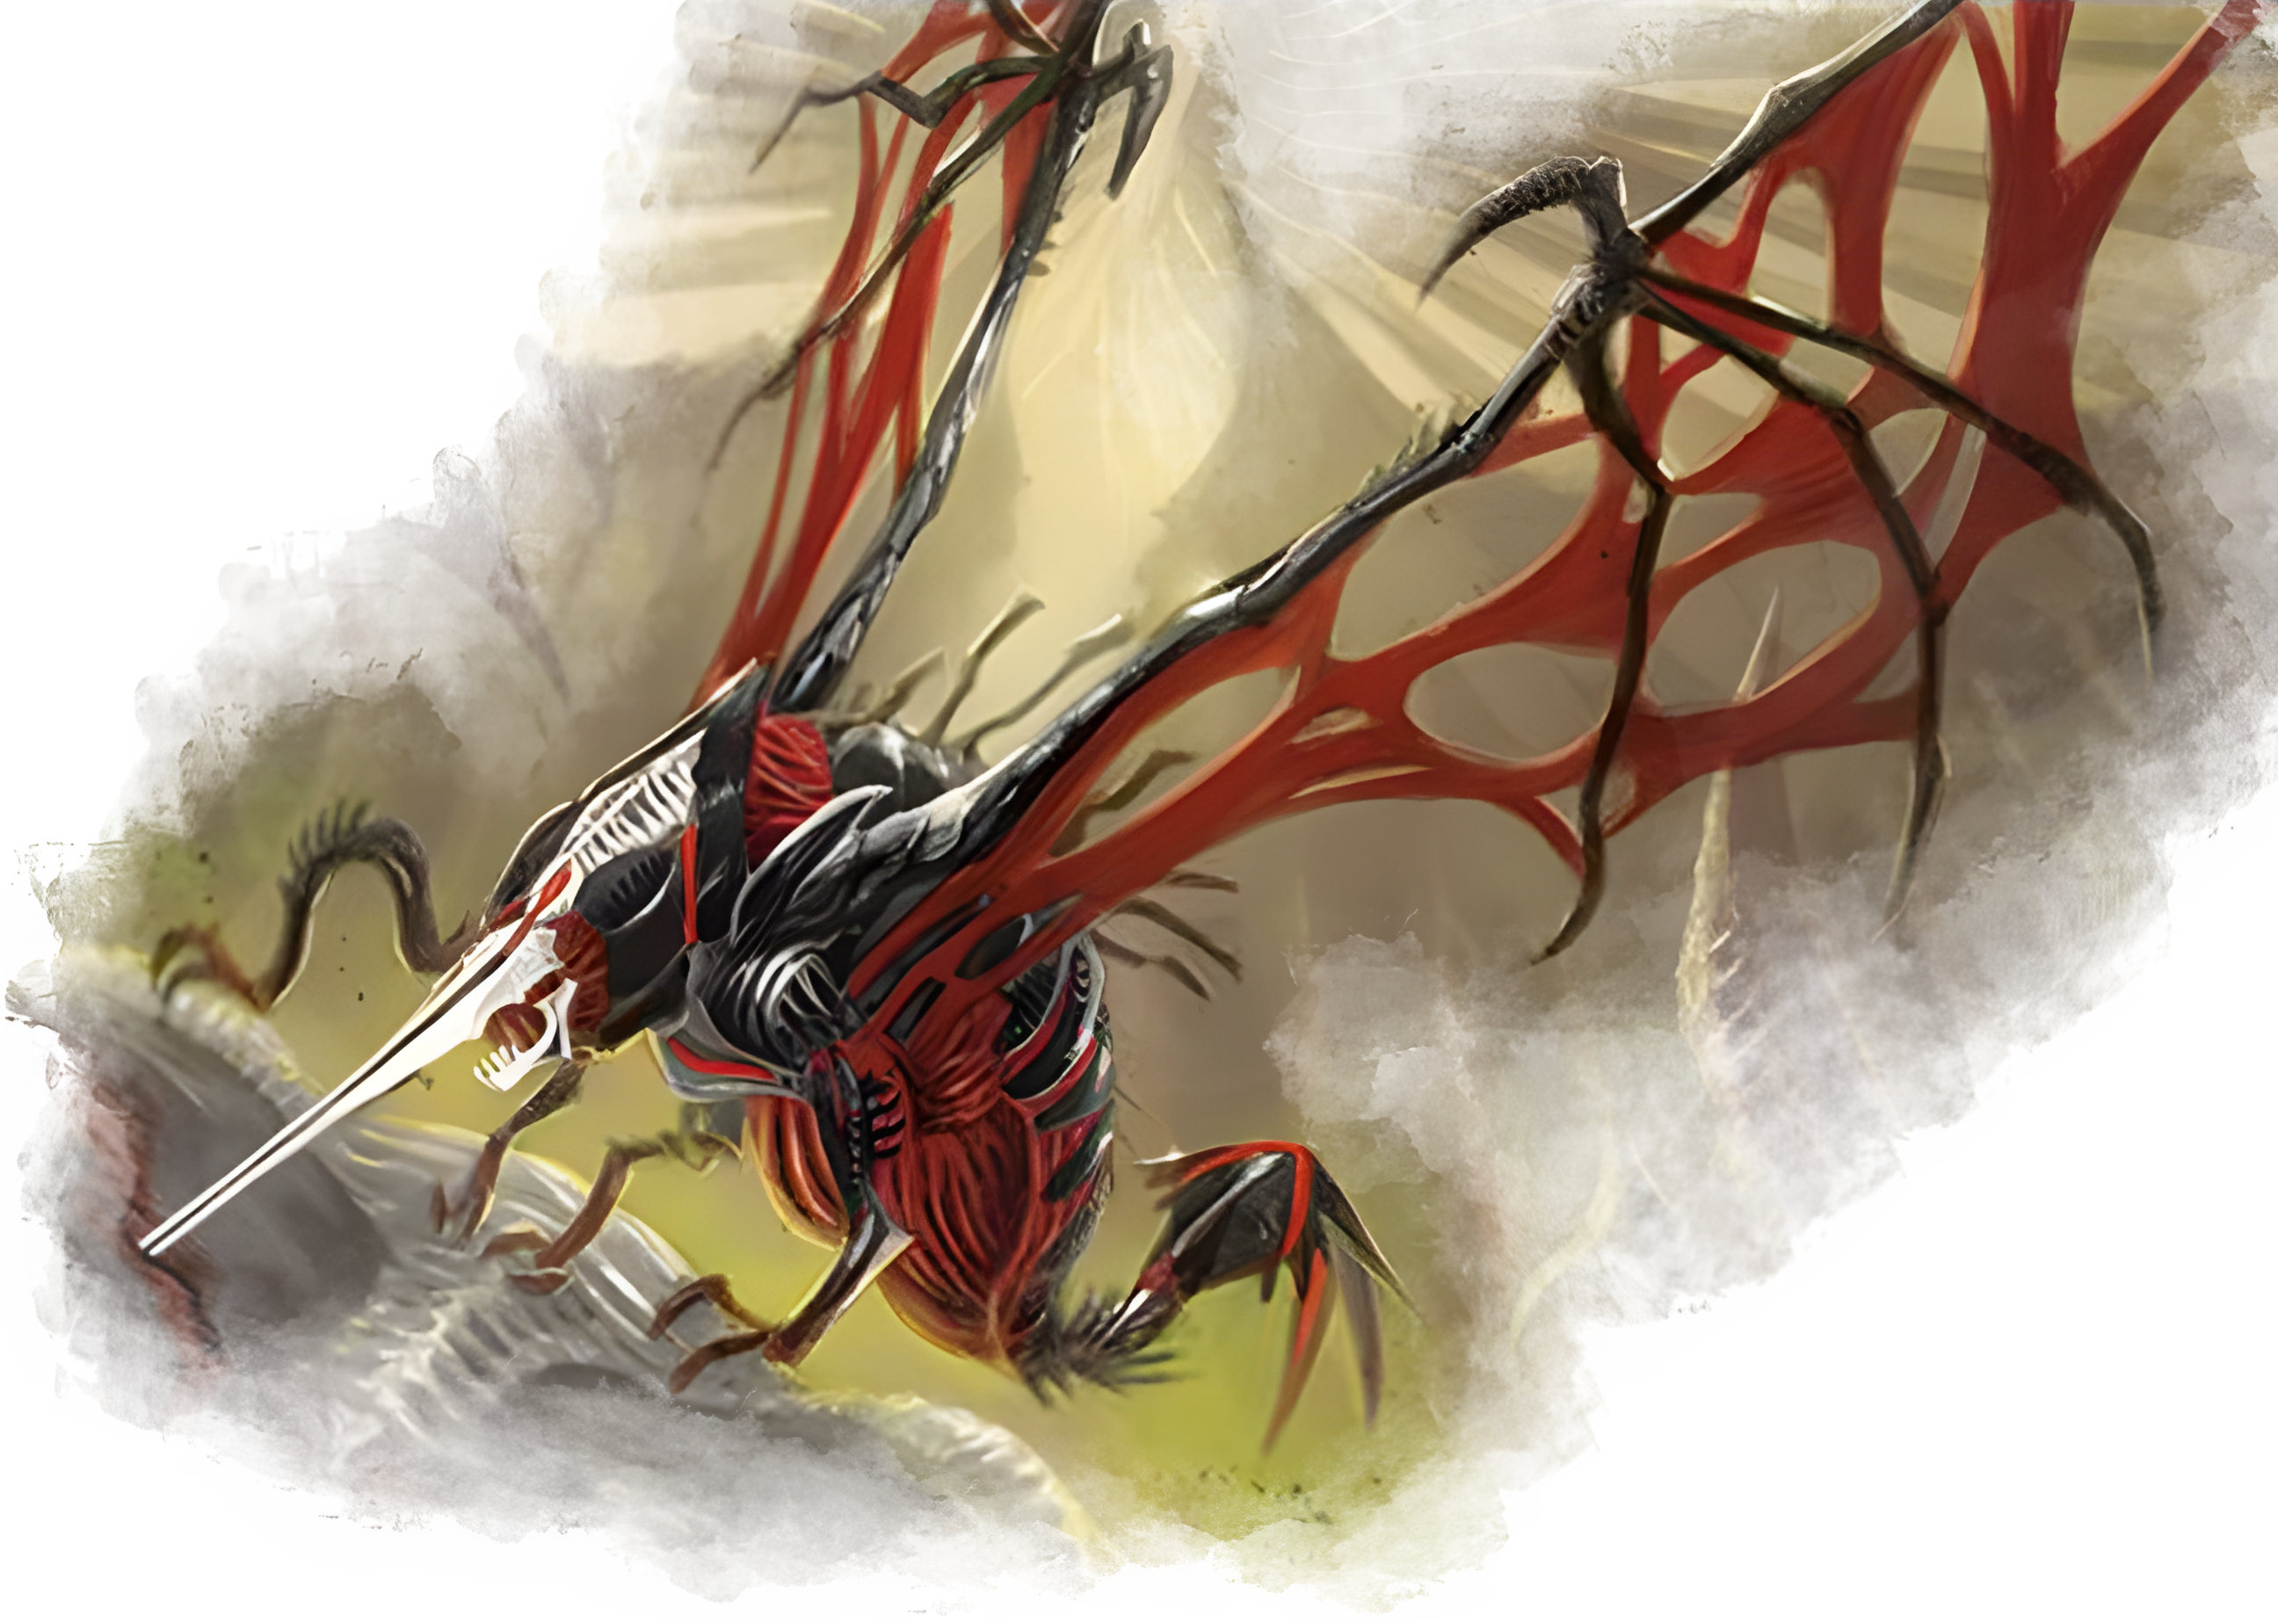
\includegraphics[width=\columnwidth, height=150pt, keepaspectratio]{Winged_Hemovoric_Venomite(2).png}};%
\end{tikzpicture}\vspace*{-2cm}%
\addImageDBEntry{Page 2}{Art}{https://scryfall.com/card/one/100/necrosquito}{Necrosquito MtG Art from Phyrexia: All Will Be One}{Abz J Harding}%

\nopagebreaksection{Venomite Lair} % section that does not induce a new page
\addcontentsline{toc}{section}{Venomite Lair}

The Hemovoric Venomite,\\a fearsome and macabre\\creature, dwells in the\\darkest corners of the\\world. This elusive and\\sinister predator pos-\\sesses a unique and gruesome\\method of reproduction. Its lair, a scene straight out of a nightmare, reflects its eerie nature.

Entering the lair of the Hemovoric Venomite feels like stepping into a crypt of decay and death. The air is thick with the stench of rotting flesh, causing even the bravest souls to recoil in disgust. Walls, adorned with ancient cobwebs and shadows that dance ominously, that seem to whisper tales of the horrors that have unfolded within.

At the heart of the lair lies a grotesque mound composed of bodies and corpses, meticulously collected by the Hemovoric Venomite. This mound serves a disturbing purpose - it is the breeding ground for its offspring. With great care, the creature selects the diseased and decaying, aware that their rotting flesh will provide sustenance for its young, forming a morbid nest of death.

Within the depths of this ghastly mound, small and vile creatures known as venomites begin to hatch. These repugnant beings, birthed from the tainted flesh of the fallen, possess an insatiable hunger for disease and decay. They feast upon the putrid remains, growing stronger with each morsel they consume.

The lair itself is dimly lit, with only a faint glow emanating from bioluminescent fungi that sprout sporadically on the walls. The flickering illumination casts eerie shadows, making it difficult to discern what lurks in the corners.

Every sound echoes through the lair, heightening the sense of dread that permeates the air. The silence is occasionally broken by the gnawing of the venomites as they feast, creating a haunting symphony of grotesque feasting.

Visitors who dare to enter the lair of the Hemovoric Venomite should be prepared for a chilling experience that will haunt their nightmares. The combination of decay, \linebreak\hspace*{1.75cm}death, and the incessant feeding of the \linebreak\hspace*{2.5cm}venomites creates an atmosphere of pure \linebreak\hspace*{4cm} horror, leaving a lasting \linebreak\hspace*{4.5cm} impression on all who witness \linebreak\hspace*{5cm} its macabre existence. \linebreak
